\section{Objetivo}

\begin{itemize}
    \item[$\blacksquare$] Obter o calor específico da água.
\end{itemize}

\section{Introdução}

Calor específico é uma grandeza física intensiva que define a variação térmica de determinada substância ao receber determinada quantidade de calor. Também é chamado de capacidade térmica mássica. A unidade no SI é J/(kg.K) (joule por quilograma e por kelvin). Uma unidade usual bastante utilizada para calores específicos é cal/(g °C) (caloria por grama e por grau Celsius). \cite{wiki:calor}

\section{Metodologia}



\subsection{Materiais Utilizados}

\begin{itemize}
    \item[$\blacksquare$] Calorímetro elétrico (com o resistor)
    \item[$\blacksquare$] Fonte
    \item[$\blacksquare$] Cronômetro
    \item[$\blacksquare$] Termômetro
\end{itemize}

\subsection{Procedimentos}

Em um ambiente isolado foi colocado um recipiente com água onde inseriu-se um calorímetro elétrico conectado a um amperímetro juntamente com um agitador e um termômetro afim de medir a variação de temperatura com o tempo, como mostra a Figura \ref{fig:calorimetro}.

\begin{figure} [htbp!]
    \centering
    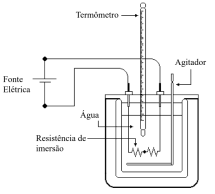
\includegraphics{figure/estrutura.png}
    \caption{Calorímetro elétrico}
    \label{fig:calorimetro}
\end{figure}

Sabendo que a corrente que passa por esse calorímetro é de $0,99\pm0,01$A, a tensão de $3,0\pm0,1$V e a massa da água de $136\pm2$g, deseja-se calcular o calor específico da água.

\section{Resultados e Discussões}

A partir do vídeo disponibilizado pelo professor, chegamos nas medidas conforme a Tabela \ref{tab:dados}.

\begin{table}[htbp!]
    \centering
    \begin{tabular}{c|c}
    \hline
    $\Delta T [\pm0,1^{\circ}C]$ & $\Delta t[\pm 0,5s]$\\
    \hline
       27   & 0    \\
27,1 & 121  \\
27,2 & 138  \\
27,3 & 151  \\
27,5 & 202  \\
27,6 & 230  \\
27,8 & 269  \\
27,9 & 303  \\
28   & 334  \\
28,1 & 356  \\
28,2 & 376  \\
28,3 & 415  \\
28,5 & 442  \\
28,6 & 479  \\
28,8 & 502  \\
28,9 & 539  \\
29   & 563  \\
29,1 & 601  \\
29,2 & 629  \\
29,3 & 664  \\
29,5 & 684  \\
29,6 & 701  \\
29,8 & 753  \\
29,9 & 783  \\
30   & 811  \\
30,1 & 834  \\
30,2 & 874  \\
30,3 & 896  \\
30,5 & 938  \\
30,6 & 965  \\
30,8 & 991  \\
30,9 & 1024 \\
31   & 1040 \\
31,1 & 1059 \\
\hline
    \end{tabular}
    \caption{Dados retirados do vídeo}
    \label{tab:dados}
\end{table}

Foi feito um gráfico de $\Delta T$ vs $\Delta t$ para estudarmos o comportamento do problema conforme a Figura \ref{fig:grafico1}.

\begin{figure} [htbp!]
    \centering
    \fbox{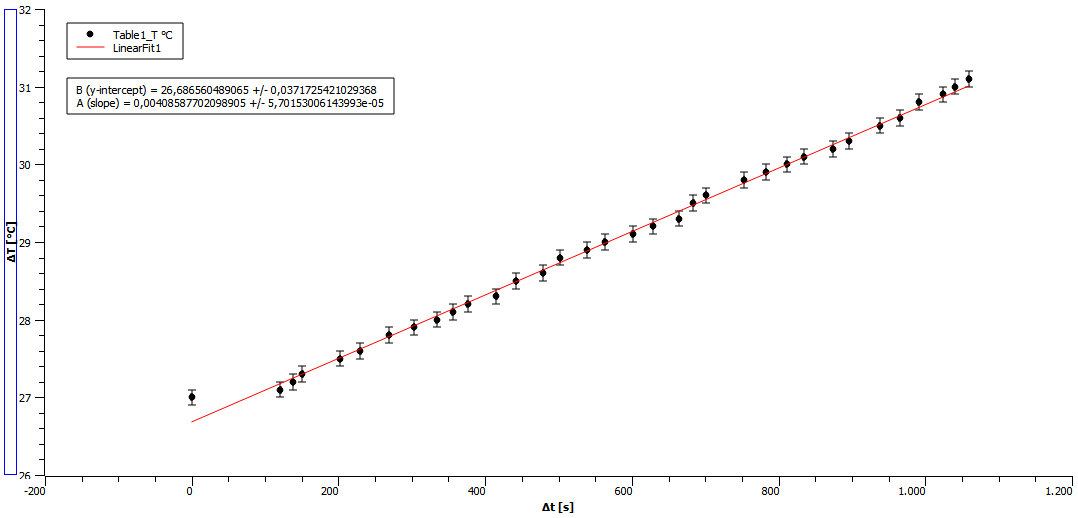
\includegraphics[width=15cm]{figure/grafico.png}}
    \caption{Gráfico $\Delta T$ vs $\Delta t$}
    \label{fig:grafico1}
\end{figure}

Considerando a equação linear

\begin{equation} \label{eq:deltat}
    \boxed{T=T_0+\frac{Vi}{mc}\Delta t}
\end{equation}

\noindent podemos calcular o calor específico pela regressão linear obtida. Considerando todas as propagações de erros, tem-se o calor específico da água de $5353 \pm 78,97\frac{J}{kg}$.

\begin{equation}
    \boxed{\frac{Vi}{mc}=A \Leftrightarrow c=\frac{Vi}{mA}}
\end{equation}

Percebe-se uma boa precisão para B, mas o valor obtido para A, usado para chegar no valor do calor específico da água, difere muito do real ($4186\frac{J}{kg}$). Necessita-se então incluir um fator desprezado na Equação \ref{eq:deltat}: a capacidade térmica do material do calorímetro.

Para essa análise, consideraremos a Equação \ref{eq:deltat1}, que inclui o fator mencionado e substituiremos o calor específico da água pelo valor correto.

\begin{equation} \label{eq:deltat1}
    \boxed{T=T_0+\frac{Vi}{mc+C_{calorímetro}}\Delta t}
\end{equation}

Onde determinaremos a capacidade térmica material do calorífico através da mesma regressão linear.

\begin{equation}
    \boxed{\frac{Vi}{mc+C_{calorímetro}}=A \Leftrightarrow C_{calorímetro}=\frac{Vi}{A}-mc}
\end{equation}

Por meio dos cálculos, considerando os erros sistemáticos, foi obtido um valor de $158,65\pm 13,07\frac{J}{C^{\circ}}$ para $C_{calorímetro}$.

\section{Conclusão}

A análise foi realizada de forma a considerar fatores externos que estariam influenciando a discordância do valor obtido para o calor específico da água com o real. Concluímos que o fator mais considerável que estaria afetando esse resultado seria a capacidade térmica do material do próprio calorímetro, o qual fizemos sua medição e constatamos um melhor resultado. A dissipação de energia não interferiu significativamente os resultados, considerando que o parâmetro B da Figura \ref{fig:grafico1} bate com a temperatura inicial observada. 

